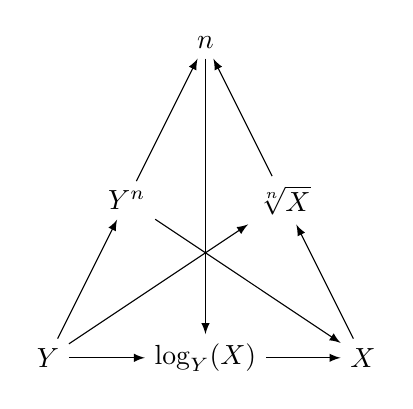
\begin{tikzpicture}[>=latex,font=\sffamily]
  % Knoten
  \node (b) at (0,0) {$Y$};
  \node (bn) at (1,2) {$Y^n$};
  \node (E) at (4,0) {$X$};
  \node (n) at (2,4) {$n$};
  \node (nrootE) at (3,2) {$\sqrt[n]{X}$};
  \node (logbE) at (2,0) {$\log_Y(X)$};

  % Pfeile
  \draw[->] (b) -- (bn) node[midway,left] {};
  \draw[->] (bn) -- (n) node[midway,left] {};
  \draw[->] (E) -- (nrootE) node[midway,right] {};
  \draw[->] (nrootE) -- (n) node[midway,right] {};
  \draw[->] (b) -- (logbE) node[midway,below] {};
  \draw[->] (logbE) -- (E) node[midway,below] {};

  % Diagonale Linien
  \draw[->] (b) -- (nrootE);
  \draw[->] (bn) -- (E);
  \draw[->] (n) -- (logbE);
  % Beschriftungen
\end{tikzpicture}